\chapter{Metodología}

En este capítulo se presenta la construcción de un modelo autorregresivo irregular de primer orden en términos
 de una secuencia $\phi_{n}$ general, para después presentar la propuesta central
de este trabajo de investigación, que consiste básicamente en proponer una secuencia $\phi_{n}$ específica que permita
al modelo autorregresivo modelar autocorrelaciones negativas y positivas, teniendo en cuenta que este modelo
debe contener como caso particular el modelo \emph{AR(1)} y el modelo \emph{IAR(1) positivo}.

\section{Construyendo el modelo autorregresivo irregular}

Para construir un proceso estocástico con estructura autorregresiva irregular, suponemos que el comportamiento irregularmente espaciado es independiente de las propiedades estocásticas del proceso.

Sea ${\varepsilon_{\tau}, \tau \in \mathbb{T}}$ una secuencia iid de variables aleatorias cada una con distribución $N(0,1)$ y defino:

$X_{\tau_{1}} = W_1^{1/2} \varepsilon_{\tau_{1}}$\\
$X_{\tau_{n+1}} = \phi_{n+1} X_{t_n} +W_{n+1}^{1/2}\varepsilon_{\tau_{n+1}}$;    para $n \geq 1$\\

Aquí, $0 \leq \phi \leq 1$, $E(X_{\tau_{n}}) = 0$ y ${W_{n}}_{n\geq 1}$ es una secuencia que caracteriza los momentos del proceso así:\\

$V(X_{\tau_{1}})= W_1$ y $V(X_{\tau_{n+1}}) = \phi_{n+1}^{2}V(X_{\tau_{n}}) + W_{n+1}$\\

Ahora, bajo este modelo, calculemos $Cov(X_{\tau_{n}}, X_{\tau_{n+k}})$, esto puede hacerse mirando casos particulares

\begin{itemize}
\item si k=1

$Cov(X_{\tau_n}, X_{\tau_{n+1}}) = Cov(X_{\tau}, \phi_{n+1} X_{t_n} +W_{n+1}^{1/2}) = \phi_{n+1} Cov(X_{t_n}, X_{t_n}) = \phi_{n+1} Var(X_{t_n}) $

\item si k=2

$Cov(X_{\tau_n}, X_{\tau_{n+2}}) = Cov(X_{\tau}, \phi_{n+2} X_{t_{n+1}} +W_{n+2}^{1/2}) = \phi_{n+2} Cov(X_{t_n}, X_{t_{n+1}}) = \phi_{n+2} \phi_{n+1} Var(X_{t_n})$

\item si k=3

$Cov(X_{\tau_n}, X_{\tau_{n+3}}) = Cov(X_{\tau}, \phi_{n+3} X_{t_{n+2}} +W_{n+3}^{1/2}) = \phi_{n+3} Cov(X_{t_n}, X_{t_{n+2}}) = \phi_{n+3}\phi_{n+2} \phi_{n+1} Var(X_{t_n})$

\item Reemplazando recursivamente tenemos:
\begin{equation}
Cov(X_{\tau_n}, X_{\tau_{n+k})} = \displaystyle\prod_{i=1}^{k} \phi_{n+i}Var(X_{t_n})
\label{cov_propuesta}
\end{equation}

\end{itemize}

Para que este proceso sea estacionario, debemos demostrar que la varianza es constante en cualquier momento $\tau$, por tanto, debemos mostrar que, para $n \geq 1$; $Var(X_{\tau_{n+1}}) = Var(X_{\tau_1}) = \gamma_0$, es decir:

\begin{equation}
\phi_{n+1}^{2}\gamma_0 + W_{n+1} = W1 = \gamma_0
\label{eq_system}
\end{equation}

despejando $W_{n+1}$ de \ref{eq_system} tenemos:

\begin{equation}
W_{n+1} = \gamma_0 (1-\phi_{n+1}^2)
\label{eq:w}
\end{equation}\label{eq:w}

Finalmente, para que nuestro modelo coincida con el modelo $AR(1)$ en el momento en que $\Delta_{n+1}=1$ para todo $n$, hacemos $\gamma_0 = \frac{\sigma^2}{1-\phi^2}$

\section{Implementando propuesta}

El foco de la investigación está en generar una propuesta estable y teóricamente coherente para la secuencia $\phi_{n+1}$, después de mucho estudiarlo, llegamos a esta expresión.

\begin{equation}
\phi_{n+1} = sign(\phi)|\phi|^{\Delta_{n+1}}
\label{eq:propuesta}
\end{equation}

Si reemplazamos \ref{eq:propuesta} en \ref{eq:w} obtenemos:

\begin{equation}
W_{n+1} = \frac{\sigma^2}{1-\phi^2} \left(1-sign(\phi)^2 |\phi|^{2\Delta_{n+1}}\right)
\label{eq:w}
\end{equation}

El modelo obtenido finalmente sigue la forma:

\begin{equation}
X_{\tau_{n+1}} = sign(\phi)|\phi|^{\Delta_{n+1}} X_{t_n} + \left[\frac{\sigma^2}{1-\phi^2} \left(1-sign(\phi)^2 |\phi|^{2\Delta_{n+1}}\right)\right]^{1/2} \varepsilon_{\tau_{n+1}}
\label{eq:propuesta_modelo}
\end{equation}
 
por definición la varianza de la expresión \ref{eq:propuesta_modelo} es:

 $V(X_{\tau_{n+1}}) =  \frac{\sigma^2}{1-\phi^2}$ y $Cov(X_{\tau_n}, X_{\tau_{n+k})} = sign(\phi)^k|\phi|^{\sum_{i=1}^{k}\Delta_{n+i}}$


\section{Estudio de simulación}
Para probar el modelo propuesto se genera un escenario de simulación, donde se muestra muestra el proceso estocastico propuesto
en la ecuación \ref{eq:propuesta_modelo}, la simulación se realiza considerando $\sigma = 1$, $\phi \in (\pm 0.1 ,\pm 0.5,\pm 0.9)$ y $n \in (20, 50, 100)$ para que pueda
observarse el comportamiento irregularmente, los tiempos $t_1 , ... , t_n$ pueden ser considerados tanto regulares como iregulares con este modelo, en este caso, consideramos
$t_n - t_{n-1} \sim 1 + poisson(\lambda = 2)$ (para asegurar que no haya 0) . La sigura \ref{fig:sim1} muestra el comportamiento
de una trayectoria simulada para cada una de las combinacióndes de los parametros establecidos en el caso de $\phi > 0$, las marcas rojas en la parte de arriba del gráfico
muestran mas claramente el comportamiento irregular. La figura \ref{fig:sim2} muestra el mismo comportamiento en el caso de $\phi < 0$.
\begin{figure}[h]
    \includegraphics[width=0.6\textwidth, angle = 270]{Kap3/Fig_Cap3/sim1.eps}
    \caption{simulación del modelo IAR con coeficientes positivos}
    \label{fig:sim1}
\end{figure}


\begin{figure}[h]
    \includegraphics[width=0.6\textwidth, angle = 270]{Kap3/Fig_Cap3/sim2.eps}
    \caption{simulación del modelo IAR con coeficientes negativos}
    \label{fig:sim2}
\end{figure}